\documentclass{article}
\usepackage{preamble}


\begin{document}

\def\moonR{15pt}
\def\moonD{2cm}

Astronomy \hfill Moon Phase Project \hfill Project Due: December 2, 2022
\vspace{1em}

In this Moon Phase Project, you'll take one picture of the Moon during each of the eight phases discussed in Chapter 4. The end product will consist of two parts:

\begin{enumerate}
\setlength\itemsep{0ex}
    \item A \href{https://www.google.com/slides/about/}{Google Slides} slide show containing one slide for each picture. Each slide contains the picture, the date \& time the picture was taken, and the moon's phase (e.g., waning gibbous) in the picture.
    \item A paper or poster model of the 8 phases of the lunar cycle around Earth, as shown below. Include the date \& time you took your pictures, and use a pencil or marker to sketch each moon in accordance to its phase on that date. For inspiration, see OpenStax \href{https://openstax.org/books/astronomy-2e/pages/4-5-phases-and-motions-of-the-moon#OSC_Astro_04_05_Moon}{Figure 4.14}.
\end{enumerate}



\begin{figure}[h!]
    \centering
\begin{tikzpicture}
    \draw[fill=cyan!30] (0,0) circle (1cm) node {\large Earth};
    \draw (\moonD,0) circle (\moonR);
    \draw ({\moonD*cos(45)},{\moonD*sin(45)}) circle (\moonR);
    \draw (0,\moonD) circle (\moonR);
    \draw ({-\moonD*cos(45)},{\moonD*sin(45)}) circle (\moonR);
    \draw (-\moonD,0) circle (\moonR);
    \draw ({-\moonD*cos(45)},{-\moonD*sin(45)}) circle (\moonR);
    \draw (0,-\moonD) circle (\moonR);
    \draw ({\moonD*cos(45)},{-\moonD*sin(45)}) circle (\moonR);

    \node[red] at (7,2) {\Large Sunlight};
    \draw[ultra thick,red,->] (8,1) --++ (-2,0);
    \draw[ultra thick,red,->] (8,0) --++ (-2,0);
    \draw[ultra thick,red,->] (8,-1) --++ (-2,0);    

    % \begin{scope}
    %     \draw (10,0) rectangle (,5);
    %     \draw (10,0) circle (5cm);
    % \end{scope}
\end{tikzpicture}
\end{figure}

\section*{Project Checkpoint \#1: Spreadsheet for Observation Planning}

\textbf{Due: Oct 21, 2022}

Download the ``Stellarium Mobile -- Star Map'' app from the Google Play store. Open Stellarium and follow the steps below.

\begin{enumerate}
\setlength\itemsep{0ex}
    \item Resize the window to full screen by clicking the middle of the upper bar.
    \item Set the location settings (located upper left) to Houston, TX.
    \item Change the time (located bottom right) to about an hour before sunset. Clicking the time stamp will reveal options to change seconds, minutes, and/or hours.
    \item Face east on the horizon and advance the time by 1-hour or 1-minute intervals until the Moon is just barely above the horizon; this is the Moon rise time. Zoom in to the Moon and observe its phase. (For Moon phases, check your notes or see \href{https://openstax.org/books/astronomy-2e/pages/4-5-phases-and-motions-of-the-moon}{OpenStax Chapter 4.5}).
    Record the date, moon rise time, and moon phase.    
\end{enumerate} 

Using your student Google account, create a blank \href{https://www.google.com/sheets/about/}{Google Sheets}  spreadsheet to record your Stellarium observations. Make sure it saves in your student Google Drive for future referencing. Record 1 row of data for each day in a lunar cycle, which lasts about a month. The purpose of the 4th column is to document the best time for you to take a picture of the Moon. For example, if the Moon is rises at 9:15PM, it may be best to wait until 9:45PM, when it's higher in the sky, to observe it. If 9:45PM doesn't work for you, verify with Stellarium that the Moon is still visible at, for example, 6:15AM the following morning.

\begin{center}
\begin{tabular}{c|c|c|c}
    \textbf{Date} & \textbf{Moon rise time} & \textbf{Moon phase} & \textbf{Good time to observe} \\
    \hline
    Oct 12 & 8:47 PM & Waning Gibbous & 9:17 PM/6:15 AM\\ 
    Oct 13 & 9:27 PM & Waning Gibbous & 9:57 PM/6:15 AM\\
    \vdots & & & \\
    Nov 12 & & & \\
\end{tabular}
\end{center}

\section*{Google Slides Presentation}
Create a Google Slides presentation containing your photos. Each slide represents one of the eight Moon phases, starting with the new Moon phase and ending with the waning crescent phase. Each slide should contain the name of the Moon phase (e.g., waxing gibbous), the photo you took of the Moon in that phase, and the date and time the picture was taken.

\vspace{1em}

When your Google Slides presentation is finalized, shared it via a QR Code. The following instructions work in the Google Chrome browser. 

\vspace{1em}

In the Slides presentation, click \texttt[red]{File}, then \texttt[red]{Share}, then \texttt[red]{Publish to web}. In the \texttt[red]{Link} tab, adjust the settings as needed and copy the URL that is generated in the box. 
\vspace{1em}

\begin{minipage}{0.45\textwidth}
\centering
\fbox{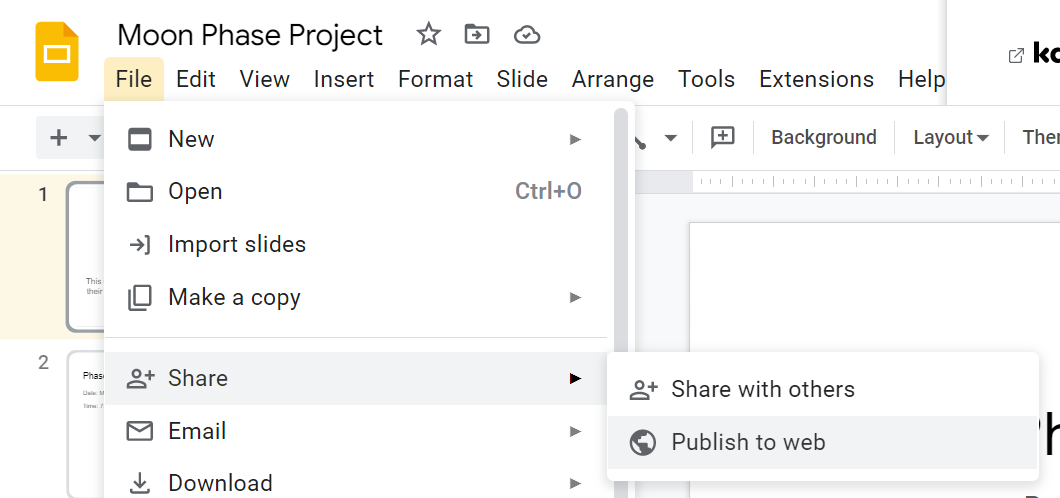
\includegraphics[width=8cm]{Figures/Slides.png}}
\end{minipage}%
\hfill
\begin{minipage}{0.45\textwidth}
\centering
\fbox{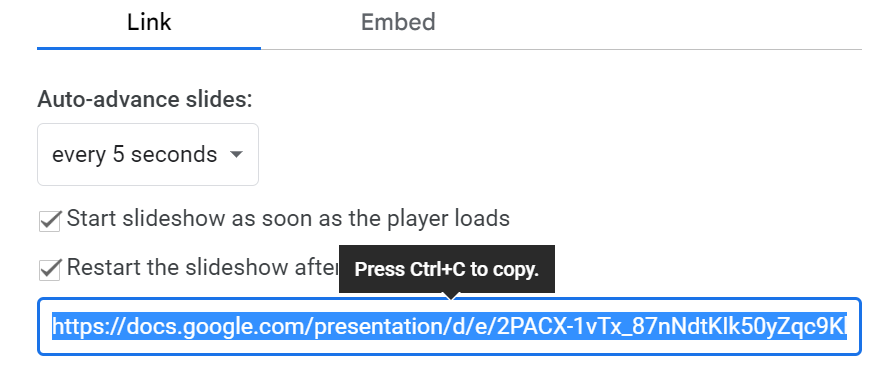
\includegraphics[width=8cm]{Figures/Slides2.png}}
\end{minipage}
\vspace{1em}

Open this URL in a new Chrome tab, to view your presentation. Right-click anywhere on the slide and click \texttt[red]{Create QR code for this page}. You may now download and print this QR code\footnote{An alternative way to create a QR code: In the far right side of the URL box at the top of the page, press the \texttt[red]{Share} icon (an arrow veering off the right, next to the bookmark star) and click \texttt[red]{Create QR Code}.} next to your Moon Phase Project for the world to see your great work.

\vspace{1em}

\begin{minipage}{0.45\textwidth}
\centering
\fbox{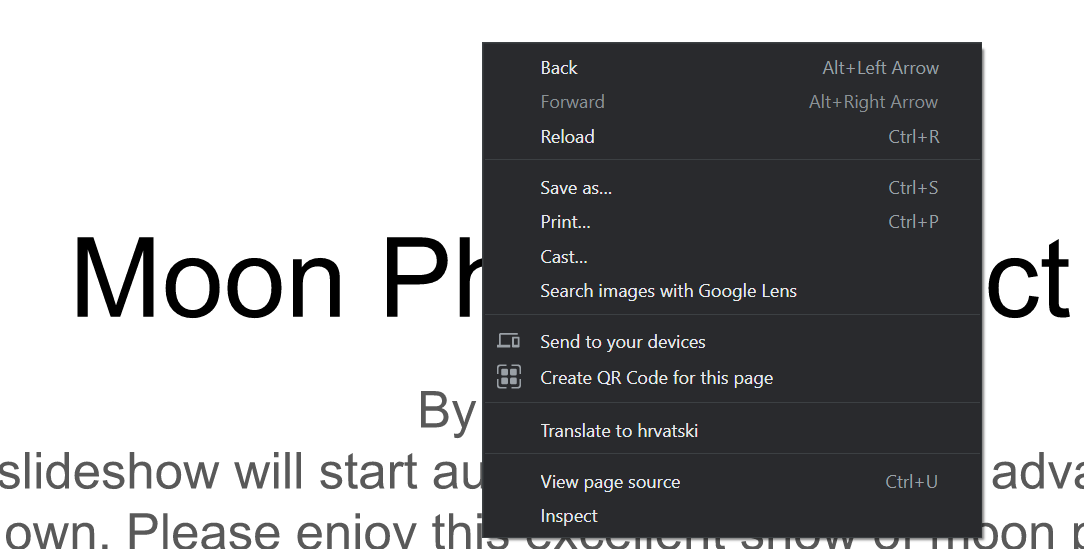
\includegraphics[width=9cm]{Figures/Slides5.png}}
\end{minipage}%
\hfill
\begin{minipage}{0.45\textwidth}
\centering
\fbox{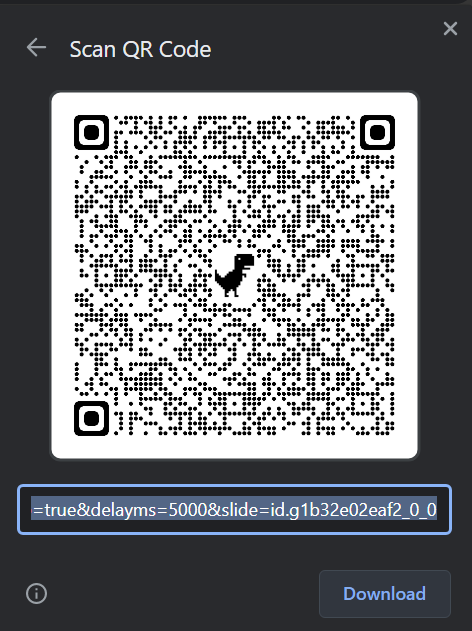
\includegraphics[width=5cm]{Figures/Slides4.png}}
\end{minipage}



\end{document}


